\documentclass{llncs}
\usepackage{makeidx}
\usepackage[pdftex]{hyperref}
\usepackage{listings}
\usepackage{graphicx}
\usepackage{color}

\definecolor{sh_comment}{rgb}{0.12, 0.38, 0.18 } %adjusted, in Eclipse: {0.25, 0.42, 0.30 } = #3F6A4D
\definecolor{sh_keyword}{rgb}{0.37, 0.08, 0.25}  % #5F1441
\definecolor{sh_string}{rgb}{0.06, 0.10, 0.98} % #101AF9

%\newfontfamily\listingsfont[Scale=0.7]{Courier} 
%\newfontfamily\listingsfontinline[Scale=0.8]{Courier New} 

\lstdefinelanguage{Xtext}{
 morekeywords={grammar, with, hidden, generate, as, import, returns, current, terminal, enum},
 keywordstyle=[2]{\textbf},
 morecomment=[l]{//}, 
 morecomment=[s]{/*}{*/}, 
 morestring=[b]",
 tabsize=4}
 
\newcommand{\lstXtext}[1]{\lstinline[breaklines=true,language=Xtext,basicstyle=\listingsfontinline,mathescape,literate={\-}{}{0\discretionary{-}{}{}}]\S#1\S}

\begin{document}
\frontmatter
\pagestyle{headings}
\title{The road to a Building Automation DSL through MDD}
\titlerunning{Building Policy Engine}
\author{Hansen, K.\, Kontostathis, K., Schmidt, E.}
\authorrunning{Hansen, K et al.}
\tocauthor{Hansen, K., Kontostathis, K., Schmidt, E.}
\institute{IT-University of Copenhagen, Denmark,\\
\email{kben@itu.dk}, \email{kkon@itu.dk}, \email{eker@itu.dk}}
\maketitle

\begin{abstract}
Modern buildings often consists of many different types of sensors and actuators. It is a complex task to control and manage them, especially when aiming for optimal energy efficiency and human comfort. If easily specified automated control of buildings is achievable, the result would be reduction in energy usage and natural resources like gas and water. We specify a buildings automation DSL based on requirements obtained from interviews with several large companies, and build it using Eclipse Modeling Framework and XText. The DSL is validated by implementing all the discovered policies.
\end{abstract}

\section{Introduction}
Energy and natural resources are precious commodities. In~\cite{janssen2004towards} it is stated that residential buildings use about 89\% of the total energy consumption for space heating, cooling and water heating. Electrical appliances uses 11\%. Other buildings use 79\% of the total energy consumption for space heating, cooling, water heating and lighting. Manually controlling buildings for energy efficiency and optimal human comfort is a time-consuming and inefficient task, if even possible. The controller has to be knowledgeable in a lot of different equipment as well as be well informed about the building. Modern buildings today often come equipped with a suite of sensors and actuators, opening up for a degree of customizable control. Building automation is therefore not only possible, but also needed. \textit{"Worldwide, there is no doubt that efficient energy saving is only possible with modern BA based on networking in all levels of abstraction."}~\cite{dietrich2010communication}. Constructing resource efficient buildings makes sense, both in a political and economical perspective. 

Our collective need is therefore that buildings can adapt to the users and the sensor-perceived environment. This can be achieved by developing governing \textit{policies} (defined as pieces of code) based on input like semi-static data, dynamic data and sensor input, which control the actuators thereby leading to the desired building state.

Merriam-Webster defines \textit{a policy} as; "A definite course or method of action selected from among alternatives and in light of given conditions to guide and determine present and future decisions."

In this paper we interview companies regarding their need for building automation \textit{policies}.These interviews  are then analyzed and iteratively specify a DSL for building automation. Then by example, our proposed DSL can capture the needs and intended requests made during the interviews.

The structure of the paper is as follows. We will start by discussing the\nameref{sec:relatedwork} and compare it to ours. Then we will move on to~\nameref{sec:method}, followed by a section on~\nameref{sec:dsldesign}. We will then explain our~ \nameref{sec:evaluation}, and it's findings in the~\nameref{sec:discussion} section. Lastly, summing up our findings in~\nameref{sec:conclusion}.

\section{Related work}\label{sec:relatedwork}
A lot of research has already been done in home and building automation, spanning from low level communication protocols like BACnet, LonWorks and EIB/KNX~\cite{communication} to full system implementations. There exists, however, not that much work on user friendly DSL designs, where everyday building concepts is mixed with time constraints and conditional logic for building automation. 

In~\cite{smartscript} a DSL named SmartScript is developed. Based on a publish/subscribe paradigm it is intended for appliance control, and implemented with a KNX adapter. It allows grouping of devices, so it is possible for example to turn on the light and dim it using the same 'light' concept, even though the light switch and dimmer are two separate electronic components. The language features three types of statements; Action, If and Loop. There are two actions; Set and Get. Although it is possible to use the group concept, it does not seem to be possible to define the entire building with rooms based on different types. This results in a long collection of variables, even for small and simple buildings. The script also seems to be operating on a much lower abstraction level than our DSL, maybe due to it's implementation that seems to have pulled the DSL more into the direction of a GPL. 

In~\cite{habitation} there is a clear distinction between usage of the domain experts (called the Catalog View) and the domain users (called the Application view). A graphical editor is used when designing an application, by dragging and dropping types into flows that will be orderly executed. However, the user designing the application still have to get comfortable with concepts such as \textit{standard functional units}, \textit{FUnitLinks} and \textit{Scenes}. Again, our DSL is at a higher abstraction level. However, the catalog view can be considered being the current state of our metamodel, where the different concepts are defined. Our model only operates on concepts already known to people expected to work with building automation like \textit{Building, Floor, Room, Sensor, Actuator, Schedule, and Policy}. Besides form the obvious differences, our DSL is text-based, versus the graphical editor in Habitation, our flow resides in the combinatory logic derived from time schedules, room types, boolean states and conditional logic specified in the policies. This will become evident in the \nameref{sec:dsldesign} section.

In the Google sponsered Home Automation Bus - openHab~\cite{openhab} it is also possible to specify rules, running on actual implemented hardware. OpenHAB offers a whole suite of implemented protocol standards and functionalities, that includes a Xtext based script interpreter. OpenHAB's rule language is, like most other systems, very low level and does not offer the expressive benefits of a high abstraction DSL.

\section{Method}\label{sec:method}
We have tailored our method as follows;

\begin{enumerate}
	\item Interviews and analysis: We conducted open-ended interviews with people working in, or close, to FM in various Danish companies.
	\item Design and development: We designed a building automation policy DSL based on an analysis of the interviews
	\item Evaluation: We evaluated the DSL in three ways;
	\begin{enumerate}
		\item Created a DSL for each of the interviews and used the requirements as basis for evaluation of our language.
		\item Asked the interviewees to look at the DSL (If we have time!) and fill our a questionnaire
		\item Conducted sessions with students having to write different policies, and analyzed their behavior(If we have time!)
	\end{enumerate}
\end{enumerate}

\section{Interviews and analysis}\label{sec:interviews}
Since building control resides with Facility Management we found it pertinent to interview company employees within, or close, to this function. We conducted open-ended interviews with these companies and documented their content by handwritten notes. Some were recorded by audio. The main purpose of the interviews was to document;

\begin{enumerate}
	\item existing governing rules, implicit or explicit.
	\item existing, and requested, sensors and actuators.
	\item requests for new governing rules regardless of their practicality or feasibility.
\end{enumerate}

In order to gather enough material to conceptualize a proper DSL, we interviewed people from the below list of companies.\\ 

\begin{table}[htdp]
\begin{center}
\begin{tabular}{|c|c|}
	\textbf{Name}\\
	\hline 
	Br\"{u}el \& Kj\ae r\\
	Bygningsstyrelsen\\
	IT-University of Copenhagen\\
	K\o benhavns Tekniske Skole\\
	ST Aerospace - Denmark\\
	UNI-C\\
\end{tabular}
\end{center}
\label{tab:interviewees}
\caption{People from these companies were interviewed.}
\end{table}%

When conducting the interviews, we stressed that practicality or feasibility should not factor in on the requests for new governing rules. This proved hard for the interviewees. Some interviews were therefore conducted over several sessions, giving the interviewees time to think creatively. 

We only used danish and english language to give examples on existing building policies and facilitate the discovery of new, relevant ones. This was done to avoid the limitations of technology, like the expressiveness of a programming language.

We therefore base this project on the requirements defined by the professionals working in Facility Management, and use their stated policies as requirements to be implemented as grammar-passed code using the developed DSL.

\section{Design and development}\label{sec:dsldesign}
By using Eclipse~\cite{eclipse}, EMF~\cite{emf} and Xtext~\cite{xtext} we have built a domain specific language that is rich enough to express the policies discovered in the analysis. We developed a grammar that is based on our programming experience, and believe has a consistent forthcoming syntax and conceptual constructs. We used our Policy Engine DSL editor to write the policies.

Our model is of considerable size, and consists of these core packages, differentiated in separate ECore Diagrams (can be viewed in full in \nameref{sec:appendix-a});

\begin{enumerate}
	\item Sensors. 9 classes.
	\item Actuators. 6 classes.
	\item Expression language. 6 classes.
	\item Building definition. 5 classes.
	\item Policy definition. 10 classes.
\end{enumerate}

\subsubsection{Sensors}:
\begin{figure}
	\centering
    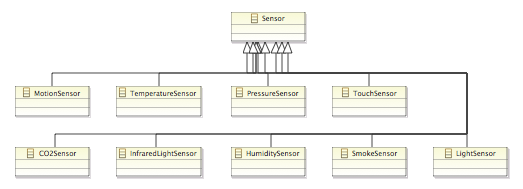
\includegraphics[scale=0.7]{ecore-sensors.png} 
	\caption{An example of \textit{Sensors} defined for a interviewee.}
	\label{fig:ecore-sensors}
\end{figure}

\pagebreak
\subsubsection{Actuators}:
\begin{figure}
	\centering
    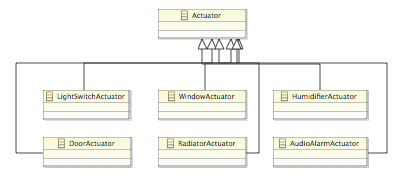
\includegraphics[scale=0.7]{ecore-actuators.png}   
	\caption{An example of \textit{Actuators} defined for a interviewee.}
	\label{fig:ecore-actuators}
\end{figure}

\subsubsection{Expression language}:
\begin{figure}
  \centering
    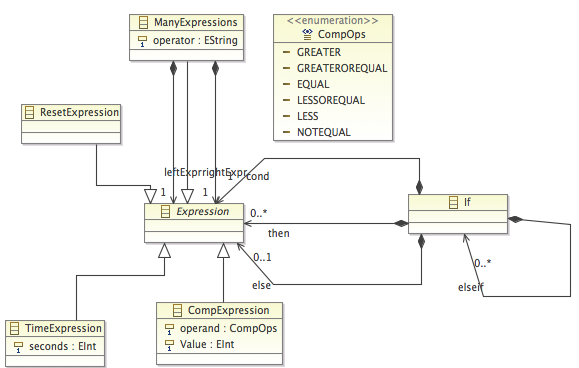
\includegraphics[width=10cm]{ecore-expression-language.png} 
	\caption{An example of \textit{expression language} defined for a interviewee.}
	\label{fig:ecore-expression-language}
\end{figure}

\pagebreak
\subsubsection{Building definition}:
\begin{figure}
  \centering 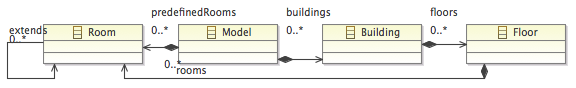
\includegraphics[scale=0.4]{ecore-building-definition.png}  
	\caption{An example of \textit{building definition} defined for a interviewee.}
	\label{fig:ecore-building-definition}
\end{figure}

\subsubsection{Policy definition}:
\begin{figure}
  \centering
    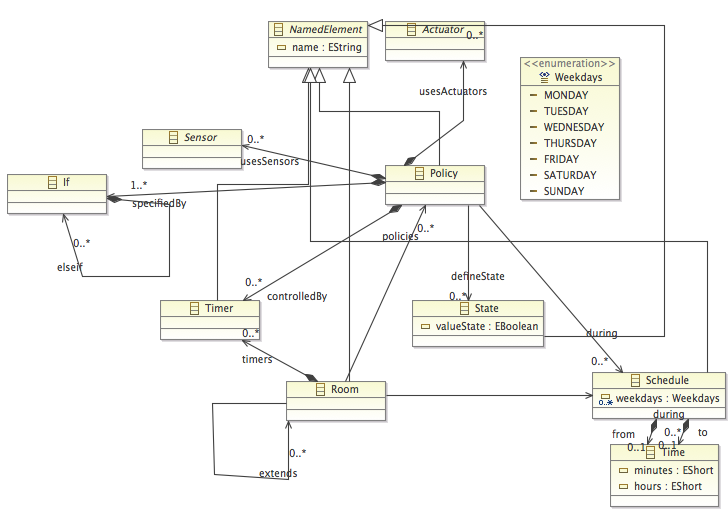
\includegraphics[scale=0.3]{ecore-policy-definition.png}	
	\caption{An example of \textit{policy definition} defined for a interviewee.}
	\label{fig:ecore-policy-definition}
\end{figure}

\pagebreak
Theres several extra classes, consisting of subsystems that can be implemented in future work.

During the analysis of the interviews, different meta-constructs was defined. It was evident that the below three key concepts was needed, in order to tailor the policies for the interviewees using DSL;

\begin{enumerate}
	\item \textit{Time}. Time have to be an integral part of the DSL, and not just in regards to internal policy logic. Several interviewees mention concepts such as; weekdays, weekends, normal working hours, holidays, night, day, morning etc.
	
	\item \textit{Building specification}. It needs to be possible to define the buildings, their floors, number and types of rooms etc.

	\item \textit{Policy}. The actual behavior, ie. adjusting actuators based on sensor input, needs to be defined. 
\end{enumerate}

\subsection{Time}\label{subsec:time}
The analysis of the interviews clearly shows that Time is necessary. We have extrapolated the need for Time in two different cases;
	\begin{enumerate}
		\item Time conditional expression - a conditional expression used for determining the flow of a behavior.
		\item Schedules - types that define a timespan that later can be attached to some behavior.
	\end{enumerate}

\subsubsection{Time conditional expression}\label{subsubsec:conditionalexpression}
A \textit{time conditional expression} is an 'if' statement that can react based on a built-in timer function. 

\begin{figure}
  \centering
    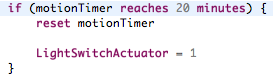
\includegraphics[width=8cm]{dsl-conditional-time-expression.png} 
	\caption{An example of a \textit{time conditional expression} that evaluates to true if more than 20 minutes have passed.}
	\label{fig:dsl-conditionalexpression}
\end{figure}

\newpage
\subsubsection{Schedules}\label{subsubsec:schedules}
\textit{Schedules} are predefined types representing a timespan where action or no-action taking place. The \textit{Schedules} can overlap, resulting in the flexibility of many policies being run in succession, which is something that almost all the interviewees requested.

\begin{figure}
  	\centering
    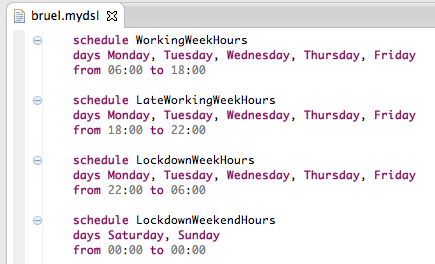
\includegraphics[width=10cm]{dsl-schedules.png}
	\caption{An example of \textit{schedules} defined for a interviewee.}
	\label{fig:dsl-schedules}
\end{figure}

\newpage
\subsection{Building specification}\label{subsec:buildingspecification}
Rooms and room types are part of the complete building specification, with terminology rooted in concepts revolving around buildings, ie. rooms, room types, floors, different sensors and actuators. \\

In order not to bother the user of the DSL with an overwhelming amount of declarations of rooms, sensors and actuators - we have designed \textit{room types} that declares static use of sensors and actuators. Independent rooms that stick out from the crown can still be defined on an instance level.

\begin{figure}
  \centering
    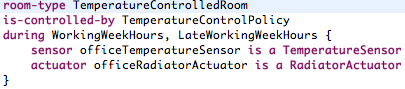
\includegraphics[width=10cm]{dsl-room-types.png}
	\caption{An example of \textit{room types} defined for a interviewee.}
	\label{fig:room-types}
\end{figure}

\newpage
Building specification as in the example below, helps up map out the actual buildings as they are in our DSL. With this we can be able to accurately define exact locations for sensors, actuator and also implement policies for specific rooms. 

\begin{figure}
  \centering
	 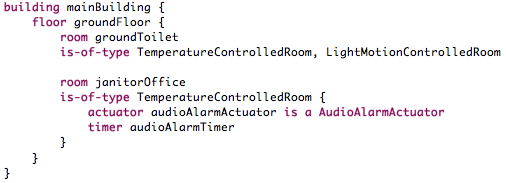
\includegraphics[width=10cm]{dsl-building-definition.png}  
	\caption{An example of \textit{building specification} defined for a interviewee.}
	\label{fig:dsl-building-definition}
\end{figure}

\newpage
\subsection{Policy}\label{subsec:policies}
Policies defines the actual behavior, ie. adjustment of actuators, based on sensor input. 

\begin{figure}
  \centering
    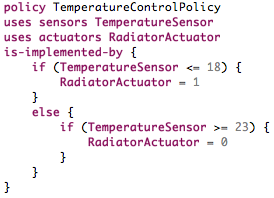
\includegraphics[width=10cm]{dsl-policy-definition.png} 
	\caption{An example of \textit{policy definition} defined for a interviewee.}
	\label{fig:dsl-policy-definition}
\end{figure}

\newpage
\section{Evaluation}\label{sec:evaluation}

\subsubsection{Br\"{u}el \& Kj\ae r}\label{subsec:bruel}

\subsubsection{Bygningstyrelsen}\label{subsec:bygstyrelsen}

\subsubsection{IT-University}\label{subsec:it-u}

\subsubsection{K\o benhavns Tekniske Skole}\label{subsec:kts}

\subsubsection{ST Aerospace}\label{subsec:st-aero}

\subsubsection{UNI-C}\label{subsec:uni-c}


\section{Discussion}\label{sec:discussion}
\subsection{Future Work}\label{subsec:futurework}
\subsubsection{Better Code Completion}\label{subsec:codecompletion}
Code completion is of great importance to our language as it is there to help guide the user in all posible options he/she has and as it is now, our DSL has code completion, which works as designed and meant to. For future work though, We would like to restrict code completion so only the declared/defined elements should be available. In \nameref{fig:code-completion} below, it shows our DSL as it is and if restricted, should only be able to have TemperatureSensor and RadiatorActuator as options for the TemperatureControlPolicy.

\begin{figure}
  \centering
    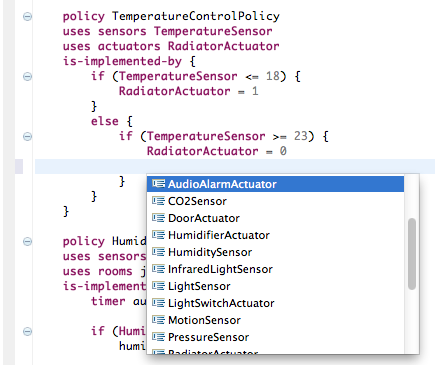
\includegraphics[width=10cm]{dsl-code-completion.png} 
	\caption{An example of \textit{code completion}.}
	\label{fig:code-completion}
\end{figure}

\subsubsection{Loop Time}\label{subsec:looptime}
Our loop is based on an outter loop that calls all policies in every iteration. Maybe it should rather be based on a priorotization of room, room-type or policies. Ex. specify that it should only run once an hour or so.

\subsubsection{Graphical Editor}\label{subsec:graphicaleditor}
Our DSL editor is currently text based and in a way requires one to have knowledge of the order in which things must be defined.

\subsubsection{Integration with existing systems}\label{subsec:integration}
In our metamodel, we have included some external systems that already exist (\textit{CTS, Access Control, Calender System and Meeting Shedule Systems}) and run in most building. Our DSL editor is currently text based.

\section{Conclusion}\label{sec:conclusion}

\bibliography{BPE}{}
\bibliographystyle{plain}

\section{Appendix A}\label{sec:appendix-a}
Because of the size of the ecore model, the xtext file, and DSL's, we have opted to have them in a repository online and are viewable by clicking the provided links.

\subsubsection{Ecore Model}\label{sec:ecore-model}
Ecore Model can be accessed by clicking the link provided below:\\ 
\url{https://github.com/rugbroed/BPE/blob/master/source/dk.itu.mdd.policyengine/model/PolicyEngine.ecorediag}

\subsubsection{PEDSL Xtext}\label{sec:xtext-pedsl}
The xtext can be viewed in full by clicking the link provided below:\\
\url{https://github.com/rugbroed/BPE/blob/master/source/PEDSL.xtext}

\subsubsection{Br\"{u}el \& Kj\ae r DSL}\label{sec:dsl-bruel}
\url{https://github.com/rugbroed/BPE/blob/master/source/PEDSL.xtext}

\subsubsection{Bygningstyrelsen DSL}\label{sec:dsl-bygstyr}
\url{https://github.com/rugbroed/BPE/blob/master/source/PEDSL.xtext}

\subsubsection{IT-University DSL}\label{sec:dsl-itu}
\url{https://github.com/rugbroed/BPE/blob/master/source/PEDSL.xtext}

\subsubsection{K\o benhavns Tekniske Skole DSL}\label{sec:dsl-kts}
\url{https://github.com/rugbroed/BPE/blob/master/source/PEDSL.xtext}

\subsubsection{ST Aerospace DSL}\label{sec:dsl-st-aero}
\url{https://github.com/rugbroed/BPE/blob/master/source/PEDSL.xtext}

\subsubsection{UNI-C DSL}\label{sec:dsl-uni-c}
\url{https://github.com/rugbroed/BPE/blob/master/source/PEDSL.xtext}

\end{document}